\documentclass[11pt]{article}
\usepackage[margin=1in]{geometry}
\usepackage{amsmath}
\usepackage{amssymb}
\usepackage{xcolor}
\usepackage{tikz}
\usetikzlibrary{positioning}
\usepackage{pgfplots}
\pgfplotsset{compat=1.18}
\usepackage{enumitem}

\title{Spring 2025 MC Problem 6: Substitution Effect Explained}
\author{ECO 310}
\date{}

\begin{document}

\maketitle

\section{The Problem}

Melsi has utility $u(B,T) = BT$ from B beef sticks and T toys. Initially, Melsi buys 16 beef sticks and 4 toys, when each beef stick costs \$1 and each toy costs \$4.

\textbf{What is the change in beef sticks due to substitution effects if the beef stick price rises to \$4?} (no change in toy price).

\begin{enumerate}
    \item[(a)] -16
    \item[(b)] -8 \quad \textcolor{red}{$\checkmark$ CORRECT}
    \item[(c)] -4
    \item[(d)] None of these is correct
\end{enumerate}

\newpage

\section{Teaching Ground: Understanding the Three Effects}

Before we solve MC6, let's build a complete understanding of how prices changes affect demand. This is one of the most important concepts in microeconomics.

\subsection{The Big Picture Question}

When the price of a good changes, how much does your consumption change?

The answer has \textbf{THREE parts}:

\begin{center}
\Large
\colorbox{blue!10}{Total Effect} = \colorbox{purple!10}{Substitution Effect} + \colorbox{orange!10}{Income Effect}
\end{center}

\subsection{Why Three Effects?}

Think about what happens when the price of beef \textbf{rises} from \$1 to \$4:

\begin{enumerate}[leftmargin=2cm]
    \item \textbf{Relative prices change:} Beef is now more expensive \textit{compared to} toys. You'll want to substitute toward the relatively cheaper good (toys). This is the \textbf{Substitution Effect}.

    \item \textbf{You're poorer:} Your money doesn't go as far. Even if you wanted to buy the same stuff as before, you can't afford it. This makes you buy less of everything (if they're normal goods). This is the \textbf{Income Effect}.

    \item \textbf{Combined impact:} These two forces work together to determine how much your consumption actually changes. This is the \textbf{Total Effect}.
\end{enumerate}

\subsection{The Three Effects Defined}

\subsubsection{Total Effect (TE)}

\begin{center}
\colorbox{yellow!30}{
\begin{minipage}{0.9\textwidth}
\textbf{Total Effect} = How much your consumption actually changes when price changes.

\vspace{0.5em}

Compare: What you bought \textbf{before} vs. what you buy \textbf{after} the price change.
\end{minipage}
}
\end{center}

\textbf{Formula:} $\text{TE} = x^{\text{new}} - x^{\text{old}}$

\textbf{Simple!} This is just the real-world change you observe.

\subsubsection{Substitution Effect (SE)}

\begin{center}
\colorbox{yellow!30}{
\begin{minipage}{0.9\textwidth}
\textbf{Substitution Effect} = How much you'd change consumption due to relative price changes, \textit{if we kept you at the same utility level}.

\vspace{0.5em}

Compare: What you bought \textbf{before} vs. what you'd buy at new prices \textbf{if compensated} to stay at original utility.
\end{minipage}
}
\end{center}

\textbf{Formula:} $\text{SE} = x^{\text{compensated}} - x^{\text{old}}$

\textbf{Key idea:} This isolates the \textit{pure} effect of the relative price change, ignoring that you're poorer.

\subsubsection{Income Effect (IE)}

\begin{center}
\colorbox{yellow!30}{
\begin{minipage}{0.9\textwidth}
\textbf{Income Effect} = How much consumption changes because you're poorer (or richer) from the price change.

\vspace{0.5em}

Compare: What you'd buy \textbf{if compensated} vs. what you \textbf{actually} buy (no compensation).
\end{minipage}
}
\end{center}

\textbf{Formula:} $\text{IE} = x^{\text{new}} - x^{\text{compensated}}$

\textbf{Key idea:} This captures the effect of losing (or gaining) purchasing power.

\subsection{The Decomposition}

These three are related by a simple equation:

\begin{center}
\Large
\fbox{
\begin{minipage}{0.8\textwidth}
\begin{align*}
\text{Total Effect} &= \text{Substitution Effect} + \text{Income Effect} \\
x^{\text{new}} - x^{\text{old}} &= (x^{\text{comp}} - x^{\text{old}}) + (x^{\text{new}} - x^{\text{comp}})
\end{align*}
\end{minipage}
}
\end{center}

Notice: The $x^{\text{comp}}$ terms cancel out, leaving $x^{\text{new}} - x^{\text{old}}$ on both sides!

\subsection{A Simple Analogy}

Imagine your favorite restaurant raises prices:

\begin{itemize}[leftmargin=2cm]
    \item \textbf{Substitution Effect:} ``This restaurant is now more expensive than the pizza place. Even if I had extra money to afford the same stuff, I'd rather get pizza now because it's relatively cheaper.''

    \item \textbf{Income Effect:} ``Also, I don't have extra money! The price increase makes me poorer, so I have to cut back on eating out in general.''

    \item \textbf{Total Effect:} Both effects combine. You eat less at the expensive restaurant, partly because you're substituting to pizza, and partly because you're just poorer overall.
\end{itemize}

\subsection{The Compensated Bundle (The Key Concept)}

The hardest part to understand is the \textbf{compensated bundle}. Let's break it down:

\subsubsection{What is it?}

The compensated bundle answers this hypothetical question:

\begin{center}
\textit{``If prices changed, but we gave you extra money to stay just as happy as before, what would you buy?''}
\end{center}

\subsubsection{Why do we care?}

Because it lets us separate two different effects:
\begin{enumerate}
    \item The effect of relative prices (substitution)
    \item The effect of being poorer/richer (income)
\end{enumerate}

Without this, we couldn't tell which effect is causing the change!

\subsubsection{Does it actually happen?}

\textbf{NO!} The compensated bundle is a \textbf{thought experiment}. In reality:
\begin{itemize}
    \item Prices change
    \item You don't get compensated
    \item You're stuck with your original income
    \item You end up at the ``new'' bundle, not the ``compensated'' bundle
\end{itemize}

The compensated bundle is just a \textbf{tool} economists use to understand what's happening.

\newpage

\subsection{Visual Guide: The Three Bundles}

Let me show you the three key bundles visually:

\begin{center}
\begin{tikzpicture}[scale=1.4]
% Axes
\draw[->] (0,0) -- (6,0) node[right] {$B$ (Beef sticks)};
\draw[->] (0,0) -- (0,6) node[above] {$T$ (Toys)};

% Original IC
\draw[thick, blue, domain=1:5.5, smooth, samples=100] plot (\x, {4/\x});
\node[blue, right] at (5.5, 4/5.5) {$u = 64$};

% New IC (lower)
\draw[thick, blue, dashed, domain=0.7:4.5, smooth, samples=100] plot (\x, {2.5/\x});

% Original budget line (steeper: slope = -1/4)
\draw[thick, red] (0, 8) -- (4.5, 6.875) node[midway, above, sloped] {\small Old: $p_B=1$};

% New budget line (flatter: slope = -1)
\draw[thick, red] (0, 8) -- (3, 5) node[midway, below, sloped] {\small New: $p_B=4$};

% Compensated budget (parallel to new, tangent to old IC)
\draw[thick, red, dashed] (0, 11.31) -- (3.5, 7.81) node[midway, above, sloped] {\small Compensated};

% Three key points
\filldraw[blue] (4, 4) circle (3pt);
\node[blue, above right] at (4, 4) {\textbf{A: Old} $(16, 4)$};

\filldraw[green!60!black] (2.83, 2.83) circle (3pt);
\node[green!60!black, left] at (2.83, 2.83) {\textbf{B: Compensated} $(8, 8)$};

\filldraw[red] (1, 1) circle (3pt);
\node[red, below left] at (1, 1) {\textbf{C: New} $(4, 4)$};

% Effect arrows
\draw[->, very thick, purple] (3.8, 3.8) -- (3, 3);
\node[purple, above] at (3.4, 3.4) {\small SE};

\draw[->, very thick, orange] (2.7, 2.7) -- (1.2, 1.2);
\node[orange, above] at (1.95, 1.95) {\small IE};

\draw[->, very thick, black, dashed] (3.8, 3.6) -- (1.3, 1.3);
\node[black, below] at (2.5, 2.5) {\small TE};

\end{tikzpicture}
\end{center}

\textbf{Key Points:}
\begin{itemize}
    \item \textbf{Point A (Old):} Where you start. Affordable and optimal at old prices.
    \item \textbf{Point B (Compensated):} Hypothetical! Where you'd be if given extra money to maintain utility at new prices.
    \item \textbf{Point C (New):} Where you actually end up. Affordable at new prices with original income.
\end{itemize}

\textbf{The Effects:}
\begin{itemize}
    \item \textbf{Purple arrow (A→B):} Substitution Effect. You substitute away from beef (now relatively expensive) toward toys.
    \item \textbf{Orange arrow (B→C):} Income Effect. Taking away the compensation makes you buy even less beef.
    \item \textbf{Black dashed arrow (A→C):} Total Effect. The real-world change you observe.
\end{itemize}

\newpage

\subsection{Step-by-Step: How to Find Each Effect}

Now let's walk through the process step-by-step using our MC6 example.

\subsubsection{Given Information}

\begin{itemize}
    \item Utility: $u(B, T) = BT$ (Cobb-Douglas)
    \item Original prices: $p_B = \$1$, $p_T = \$4$
    \item Original bundle: $(B, T) = (16, 4)$
    \item Original income: $m = 1(16) + 4(4) = \$32$
    \item New price: $p_B = \$4$ (beef price rises!)
\end{itemize}

\subsubsection{Step 1: Find Original Utility}

$$u^* = 16 \times 4 = 64$$

This is our target utility for the compensated bundle.

\subsubsection{Step 2: Find the Compensated Bundle}

\textbf{Question:} At the new prices $(p_B=4, p_T=4)$, what bundle achieves $u=64$ most cheaply?

This is a Hicksian demand problem!

\textbf{Tangency condition:} For Cobb-Douglas with equal exponents:
$$\frac{MU_B}{MU_T} = \frac{p_B}{p_T} \quad \Rightarrow \quad \frac{T}{B} = \frac{4}{4} = 1 \quad \Rightarrow \quad T = B$$

\textbf{Utility constraint:}
$$BT = 64 \quad \text{and} \quad T = B \quad \Rightarrow \quad B^2 = 64 \quad \Rightarrow \quad B = 8$$

Therefore: $\boxed{(B^{\text{comp}}, T^{\text{comp}}) = (8, 8)}$

\subsubsection{Step 3: Find the New Bundle}

\textbf{Question:} At new prices $(p_B=4, p_T=4)$ with income $m=32$, what do you buy?

This is a Marshallian demand problem!

With Cobb-Douglas and equal exponents, spend half income on each good:
$$B^{\text{new}} = \frac{m/2}{p_B} = \frac{16}{4} = 4$$
$$T^{\text{new}} = \frac{m/2}{p_T} = \frac{16}{4} = 4$$

Therefore: $\boxed{(B^{\text{new}}, T^{\text{new}}) = (4, 4)}$

\subsubsection{Step 4: Calculate the Three Effects}

\textbf{Substitution Effect:}
$$\text{SE} = B^{\text{comp}} - B^{\text{old}} = 8 - 16 = \boxed{-8}$$

\textbf{Income Effect:}
$$\text{IE} = B^{\text{new}} - B^{\text{comp}} = 4 - 8 = \boxed{-4}$$

\textbf{Total Effect:}
$$\text{TE} = B^{\text{new}} - B^{\text{old}} = 4 - 16 = \boxed{-12}$$

\textbf{Check:} $\text{SE} + \text{IE} = -8 + (-4) = -12 = \text{TE}$ $\checkmark$

\newpage

\subsection{Understanding the Signs}

\subsubsection{Why is SE Negative?}

When the price of beef rises, beef becomes \textbf{relatively more expensive} compared to toys. Even if we compensate you to stay at the same utility, you'll substitute away from beef toward the relatively cheaper toys.

\begin{center}
\colorbox{green!20}{
\textbf{Key Rule:} Substitution Effect is \textbf{ALWAYS} negative (or zero) for a price increase.
}
\end{center}

This is called the \textbf{Law of Compensated Demand}.

\subsubsection{Why is IE Negative?}

Beef is a \textbf{normal good}. This means when you get richer, you buy more beef; when you get poorer, you buy less beef.

The price increase makes you effectively poorer. Going from the compensated bundle (where you're given extra money) to the new bundle (where you're not) means losing that extra money. Since beef is normal, you buy less.

\begin{center}
\colorbox{yellow!30}{
\begin{minipage}{0.9\textwidth}
\textbf{For Normal Goods:} When price rises, IE is negative (reinforces SE).

\textbf{For Inferior Goods:} When price rises, IE is positive (opposes SE).
\end{minipage}
}
\end{center}

\subsubsection{The Combined Effect}

Both effects are negative, so they \textbf{work together}:
\begin{itemize}
    \item SE pulls beef consumption down by 8 (substitution away)
    \item IE pulls it down by another 4 (you're poorer)
    \item Total: beef consumption falls by 12
\end{itemize}

\subsection{Common Questions}

\subsubsection{Q: Why not just calculate Total Effect directly?}

\textbf{A:} We can! But breaking it into SE and IE helps us understand \textit{why} consumption changes. It tells us:
\begin{itemize}
    \item How much is due to relative prices (pure substitution)?
    \item How much is due to income/purchasing power?
\end{itemize}

This is especially important for policy analysis, welfare economics, and understanding different types of goods.

\subsubsection{Q: Does the compensated bundle ever actually happen?}

\textbf{A:} No! It's purely hypothetical. We use it as an analytical tool. In reality:
\begin{itemize}
    \item Prices change
    \item Your income doesn't automatically adjust
    \item You move directly from Old → New
\end{itemize}

The compensated bundle is the intermediate step we imagine to separate the two effects.

\subsubsection{Q: What if the price falls instead of rises?}

\textbf{A:} The same logic applies, but signs flip:
\begin{itemize}
    \item SE would be positive (substitute toward the now-cheaper good)
    \item IE would be positive for normal goods (you're richer)
    \item Both effects reinforce, so TE is positive (buy more)
\end{itemize}

\subsubsection{Q: Can Total Effect ever be positive when price rises?}

\textbf{A:} Yes, for \textbf{Giffen goods}! These are strongly inferior goods where:
\begin{itemize}
    \item SE is negative (substitute away) — always true
    \item IE is positive and large (inferior good, and you're poorer means buy more)
    \item If $|$IE$| > |$SE$|$, then TE is positive
\end{itemize}

This is rare in practice but theoretically possible.

\subsection{Summary Table}

\begin{center}
\begin{tabular}{|l|p{6cm}|c|}
\hline
\textbf{Effect} & \textbf{What It Measures} & \textbf{MC6 Value} \\
\hline
\textbf{SE} & Change due to relative prices, holding utility constant & $-8$ \\
\hline
\textbf{IE} & Change due to purchasing power, at new relative prices & $-4$ \\
\hline
\textbf{TE} & Total actual change observed in real world & $-12$ \\
\hline
\end{tabular}
\end{center}

\vspace{1em}

\begin{center}
\colorbox{blue!10}{
\Large
\textbf{Total Effect = Substitution Effect + Income Effect}
}
\end{center}

\newpage

\section{What the Hell is the Substitution Effect?}

When a price changes, your demand changes for \textbf{TWO reasons}:

\begin{enumerate}
    \item \textbf{Substitution Effect (SE):} The good became relatively more/less expensive, so you substitute toward the cheaper good \textit{(holding utility constant)}

    \item \textbf{Income Effect (IE):} The price change affects your purchasing power, making you richer or poorer
\end{enumerate}

\subsection{Key Definition}

\begin{center}
\colorbox{yellow!30}{
\begin{minipage}{0.9\textwidth}
\textbf{Substitution Effect} = Change in demand when you \textbf{compensate} the consumer to stay at the \textbf{same utility level} after the price change.
\end{minipage}
}
\end{center}

\textbf{In other words:} If we gave you just enough money to get back to your original utility level after the price increase, how would your consumption change?

\section{The Slutsky Decomposition}

When price $p_1$ changes, the total change in demand can be split:

$$\boxed{\underbrace{x_1^{\text{new}} - x_1^{\text{old}}}_{\text{Total Effect}} = \underbrace{x_1^c - x_1^{\text{old}}}_{\text{Substitution Effect}} + \underbrace{x_1^{\text{new}} - x_1^c}_{\text{Income Effect}}}$$

where $x_1^c$ is the \textbf{compensated demand} (Hicksian demand at new prices, old utility).

\section{Graphical Intuition}

\begin{center}
\begin{tikzpicture}[scale=1.3]
% Axes
\draw[->] (0,0) -- (6,0) node[right] {$B$ (Beef sticks)};
\draw[->] (0,0) -- (0,6) node[above] {$T$ (Toys)};

% Original indifference curve (u = 64)
\draw[thick, blue, domain=1:5.5, smooth, samples=100] plot (\x, {4/\x});
\node[blue, right] at (5.5, 4/5.5) {$u = 64$};

% New indifference curve (lower utility, u = 16)
\draw[thick, blue, dashed, domain=0.7:4.5, smooth, samples=100] plot (\x, {2.5/\x});
\node[blue, below] at (4.5, 2.5/4.5) {$u = 16$ (new)};

% Original budget line (slope = -1/4)
\draw[thick, red] (0, 8) -- (32, 0);
\node[red, above, rotate=-7] at (10, 5.5) {Original: $p_B=1, p_T=4$};

% New budget line (slope = -1, same income m=32)
\draw[thick, red] (0, 8) -- (8, 0);
\node[red, above left, rotate=-45] at (5, 3) {New: $p_B=4, p_T=4$};

% Compensated budget line (parallel to new, tangent to old IC)
\draw[thick, red, dashed] (0, 11.31) -- (11.31, 0);
\node[red, above, rotate=-45] at (8, 3.31) {\small Compensated};

% Points
\filldraw[black] (4, 4) circle (2pt) node[above right] {A: Original $(16, 4)$};
\filldraw[black] (2.83, 2.83) circle (2pt) node[above left] {B: Compensated $(8, 8)$};
\filldraw[black] (1, 1) circle (2pt) node[below right] {C: New $(4, 4)$};

% Arrows showing effects
\draw[->, thick, purple, >=stealth] (3.7, 3.5) -- (3, 3);
\node[purple, below] at (3.3, 3.2) {\small SE};

\draw[->, thick, orange, >=stealth] (2.6, 2.6) -- (1.3, 1.3);
\node[orange, below] at (2, 2) {\small IE};

\draw[->, thick, black, >=stealth] (3.8, 3.7) -- (1.5, 1.5);
\node[black, above] at (2.7, 2.7) {\small Total};

% Grid lines for reference
\draw[dotted, gray] (4, 0) -- (4, 4);
\draw[dotted, gray] (2.83, 0) -- (2.83, 2.83);
\draw[dotted, gray] (1, 0) -- (1, 1);
\node[below] at (4, 0) {16};
\node[below] at (2.83, 0) {8};
\node[below] at (1, 0) {4};

\end{tikzpicture}
\end{center}

\textbf{Key Points:}
\begin{itemize}
    \item \textbf{A}: Original optimal bundle at old prices
    \item \textbf{B}: Compensated bundle (new prices, but enough income to maintain $u=64$)
    \item \textbf{C}: New optimal bundle at new prices and original income
    \item \textbf{A $\to$ B}: Substitution Effect (what MC6 asks for)
    \item \textbf{B $\to$ C}: Income Effect
    \item \textbf{A $\to$ C}: Total Effect
\end{itemize}

\section{Step-by-Step Solution}

\subsection{Step 1: Find Original Utility}

Original bundle: $(B, T) = (16, 4)$ at prices $(p_B, p_T) = (1, 4)$

$$u^* = B \times T = 16 \times 4 = 64$$

Original income: $m = p_B \cdot B + p_T \cdot T = 1(16) + 4(4) = 32$

\subsection{Step 2: Understand New Prices}

After the price change:
\begin{itemize}
    \item $p_B^{\text{new}} = 4$ (was \$1, now \$4)
    \item $p_T^{\text{new}} = 4$ (unchanged)
    \item Income still $m = 32$ (no actual compensation yet)
\end{itemize}

\subsection{Step 3: Find Optimal Allocation Condition at New Prices}

For Cobb-Douglas $u(B, T) = BT$ with equal exponents, the optimal allocation satisfies:
$$\frac{MU_B}{MU_T} = \frac{p_B}{p_T}$$

Calculate marginal utilities:
$$MU_B = \frac{\partial u}{\partial B} = T$$
$$MU_T = \frac{\partial u}{\partial T} = B$$

Therefore:
$$\frac{T}{B} = \frac{p_B}{p_T} = \frac{4}{4} = 1$$

This gives us:
$$\boxed{T = B}$$

At the new prices, Melsi optimally consumes equal amounts of beef sticks and toys.

\subsection{Step 4: Find Compensated Bundle (Substitution Effect)}

For the substitution effect, we want the bundle that:
\begin{enumerate}
    \item Achieves the \textbf{original utility} $u^* = 64$
    \item Is optimized at the \textbf{new prices} (so $T = B$)
\end{enumerate}

This is the \textbf{Hicksian demand} at new prices for utility $u^* = 64$.

Using $T = B$ and $u = BT = 64$:
\begin{align*}
B \cdot T &= 64 \\
B \cdot B &= 64 \quad \text{(substitute } T = B \text{)} \\
B^2 &= 64 \\
B^c &= 8
\end{align*}

Therefore: $T^c = 8$ as well.

\textbf{Compensated bundle:} $(B^c, T^c) = (8, 8)$

\subsection{Step 5: Calculate Substitution Effect}

$$\text{Substitution Effect} = B^c - B^{\text{original}} = 8 - 16 = \boxed{-8}$$

The answer is \textbf{(b): -8 beef sticks}.

\section{Why is the Substitution Effect Negative?}

Beef sticks became \textbf{4 times more expensive} (from \$1 to \$4). Even if we compensate Melsi to stay at the same utility level, she will substitute \textbf{away from beef sticks} (now expensive) and \textbf{toward toys} (relatively cheaper now).

The substitution effect is \textbf{always negative} for a price increase. This is called the \textbf{Law of Compensated Demand}.

\section{Complete Slutsky Decomposition}

Let's find the \textbf{total effect} and \textbf{income effect} too.

\subsection{Find Actual New Bundle}

With new prices $(p_B, p_T) = (4, 4)$ and original income $m = 32$, using Cobb-Douglas with equal exponents (spend half income on each good):

$$B^{\text{new}} = \frac{m/2}{p_B} = \frac{16}{4} = 4$$
$$T^{\text{new}} = \frac{m/2}{p_T} = \frac{16}{4} = 4$$

New bundle: $(B^{\text{new}}, T^{\text{new}}) = (4, 4)$

New utility: $u^{\text{new}} = 4 \times 4 = 16$ (much lower than original $u = 64$!)

\subsection{The Full Decomposition}

\begin{center}
\begin{tabular}{|l|c|c|}
\hline
\textbf{Effect} & \textbf{Formula} & \textbf{Value} \\
\hline
Substitution Effect & $B^c - B^{\text{old}} = 8 - 16$ & $-8$ \\
Income Effect & $B^{\text{new}} - B^c = 4 - 8$ & $-4$ \\
\hline
Total Effect & $B^{\text{new}} - B^{\text{old}} = 4 - 16$ & $-12$ \\
\hline
\end{tabular}
\end{center}

Verify: $-8 + (-4) = -12$ \checkmark

\subsection{Visual Summary}

$$\underbrace{16 \to 8}_{\text{SE: -8}} \to \underbrace{8 \to 4}_{\text{IE: -4}}$$

Both effects are negative because:
\begin{itemize}
    \item \textbf{SE is negative:} Beef became relatively more expensive, so substitute away
    \item \textbf{IE is negative:} Beef is a normal good, and the price increase made us poorer, so buy less
\end{itemize}

\section{Deep Dive: Understanding the Income Effect}

\subsection{What is ``New - Comp''?}

The Income Effect formula is:
$$\boxed{\text{Income Effect} = B^{\text{new}} - B^{\text{comp}} = 4 - 8 = -4}$$

But what does this \textbf{actually mean}? Let's break it down step by step.

\subsection{The Three-Act Story}

\textbf{Act 1: Original Situation (Point A)}

You start with:
\begin{itemize}
    \item Income: $m = 32$
    \item Prices: $p_B = 1$, $p_T = 4$
    \item Bundle: $(B, T) = (16, 4)$
    \item Utility: $u = 64$
\end{itemize}

Everything is normal. You're happy.

\textbf{Act 2: Substitution Effect $\to$ Compensated Bundle (Point B)}

The price of beef rises to \$4. We ask: \textit{``If we gave you extra money to stay at utility 64, what would you buy at the new prices?''}

This is the \textbf{compensated} scenario:
\begin{itemize}
    \item New prices: $p_B = 4$, $p_T = 4$
    \item \textbf{Compensated income:} $m^c = 64$ (we give you more money!)
    \item Bundle: $(B, T) = (8, 8)$
    \item Utility: still $u = 64$ (by design)
\end{itemize}

You consume less beef $(16 \to 8)$ because it's relatively more expensive. This is the \textbf{Substitution Effect: -8 beef sticks}.

\textbf{Key point:} Your utility hasn't changed because we compensated you with extra money.

\textbf{Act 3: Income Effect $\to$ Take Away the Compensation (Point C)}

Reality check: \textit{``Wait, we're not actually giving you that extra money. Back to your original income \$32. Now what?''}

This is the \textbf{actual} scenario:
\begin{itemize}
    \item Prices: $p_B = 4$, $p_T = 4$ (same as compensated)
    \item \textbf{Actual income:} $m = 32$ (your original income, \textbf{no compensation})
    \item Bundle: $(B, T) = (4, 4)$
    \item Utility: $u = 16$ (much lower!)
\end{itemize}

You consume even less beef $(8 \to 4)$ because you're poorer. This is the \textbf{Income Effect: -4 beef sticks}.

\subsection{What's Happening with the Income Effect?}

The income effect captures: \textbf{``You're poorer because of the price increase!''}

When we calculated the compensated bundle at Point B, we \textbf{pretended} you got extra money (income = \$64) to stay at utility 64. But in reality, you don't get that compensation. Your actual income is still $m = 32$.

So the income effect is the movement from:
\begin{itemize}
    \item \textbf{Point B (compensated, hypothetical):} ``If you had enough money to maintain utility 64...''
    \item \textbf{Point C (actual, real):} ``...but you don't, so here's what you can actually afford''
\end{itemize}

\subsection{Why is the Income Effect Negative for Beef?}

Beef is a \textbf{normal good}: when you get richer, you buy more beef; when you get poorer, you buy less.

Going from compensated (B) to actual (C) means you're effectively \textbf{getting poorer} (losing the hypothetical compensation of \$32):
\begin{itemize}
    \item Compensated income: \$64
    \item Actual income: \$32
    \item You're \$32 poorer!
\end{itemize}

Since beef is normal:
\begin{itemize}
    \item Poorer $\to$ Buy less beef
    \item IE is negative: $-4$ beef sticks
\end{itemize}

\subsection{The Compensated Bundle is Hypothetical!}

This is crucial to understand: \textbf{Point B never actually happens.}

The compensated bundle is a \textbf{thought experiment} we use as a stepping stone to separate:
\begin{enumerate}
    \item \textbf{Pure substitution (SE):} Change due to relative prices, holding utility constant
    \item \textbf{Pure income (IE):} Change due to real income, holding relative prices constant
\end{enumerate}

We use Point B to split the total effect into two interpretable pieces.

\subsection{Visual Timeline}

\begin{center}
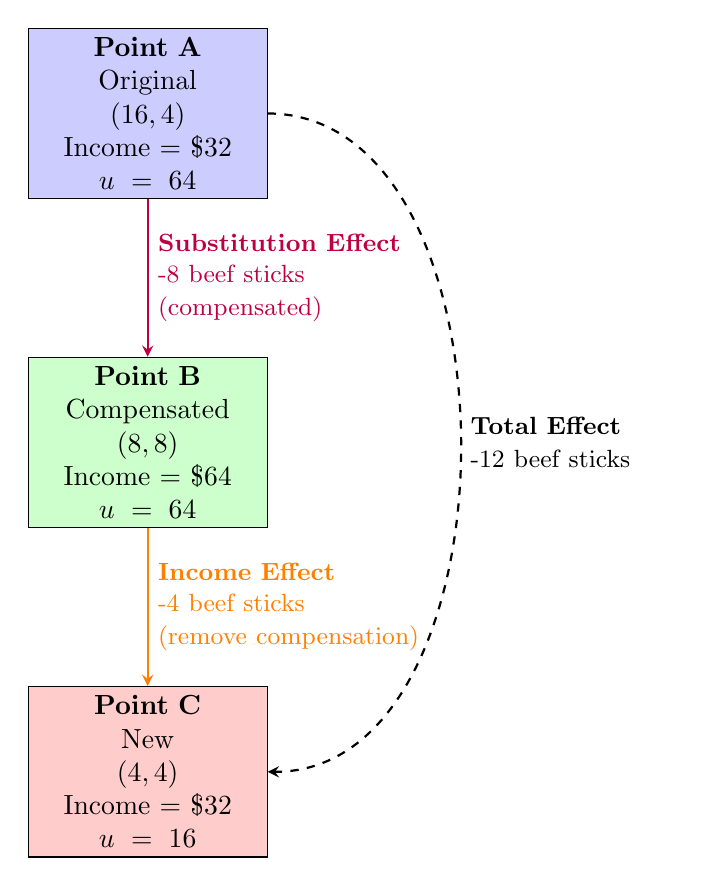
\begin{tikzpicture}[scale=1.1, node distance=2cm]
% Nodes
\node[draw, rectangle, fill=blue!20, minimum width=3cm, text width=2.8cm, align=center] (A) {
    \textbf{Point A}\\
    Original\\
    $(16, 4)$\\
    Income = \$32\\
    $u = 64$
};

\node[draw, rectangle, fill=green!20, minimum width=3cm, text width=2.8cm, align=center, below=of A] (B) {
    \textbf{Point B}\\
    Compensated\\
    $(8, 8)$\\
    Income = \$64\\
    $u = 64$
};

\node[draw, rectangle, fill=red!20, minimum width=3cm, text width=2.8cm, align=center, below=of B] (C) {
    \textbf{Point C}\\
    New\\
    $(4, 4)$\\
    Income = \$32\\
    $u = 16$
};

% Arrows
\draw[->, thick, purple, >=stealth] (A) -- (B) node[midway, right, text width=3.5cm, align=left] {\small \textbf{Substitution Effect}\\-8 beef sticks\\(compensated)};

\draw[->, thick, orange, >=stealth] (B) -- (C) node[midway, right, text width=3.5cm, align=left] {\small \textbf{Income Effect}\\-4 beef sticks\\(remove compensation)};

\draw[->, thick, black, >=stealth, dashed] (A.east) to[out=0, in=0] node[right, text width=2.5cm, align=left] {\small \textbf{Total Effect}\\-12 beef sticks} (C.east);

\end{tikzpicture}
\end{center}

\subsection{``New - Comp'' Means Taking Away the Compensation}

The formula $B^{\text{new}} - B^{\text{comp}}$ literally means:
\begin{itemize}
    \item $B^{\text{comp}} = 8$: How much beef you'd buy if compensated to stay at $u = 64$
    \item $B^{\text{new}} = 4$: How much beef you actually buy with your real income
    \item Difference $= 4 - 8 = -4$: The effect of being poorer (not getting the compensation)
\end{itemize}

\textbf{In plain English:} ``Taking away the compensation makes you 4 beef sticks poorer.''

\subsection{Income Effect for Normal vs. Inferior Goods}

The \textbf{sign} of the income effect depends on whether the good is normal or inferior:

\begin{center}
\begin{tabular}{|l|c|c|}
\hline
\textbf{Good Type} & \textbf{When Price $\uparrow$} & \textbf{Income Effect Sign} \\
\hline
Normal Good & You're poorer $\to$ Buy less & Negative (reinforces SE) \\
Inferior Good & You're poorer $\to$ Buy more & Positive (opposes SE) \\
\hline
\end{tabular}
\end{center}

For beef in our problem:
\begin{itemize}
    \item Beef is normal (when richer, buy more)
    \item Price increased $\to$ Poorer
    \item IE is negative: $-4$
\end{itemize}

\subsection{Key Takeaway}

\begin{center}
\colorbox{yellow!30}{
\begin{minipage}{0.9\textwidth}
\textbf{Income Effect = ``What happens when we stop pretending you're compensated?''}

It measures the pure effect of the change in purchasing power, \textit{after} you've already adjusted to the new relative prices.
\end{minipage}
}
\end{center}

\section{Alternative Approach: Using Expenditure Function}

For Cobb-Douglas $u = BT$ with equal exponents, the expenditure function is:
$$e(p_B, p_T, u) = 2\sqrt{p_B p_T \cdot u}$$

At new prices and original utility $u^* = 64$:
$$e(4, 4, 64) = 2\sqrt{4 \times 4 \times 64} = 2\sqrt{1024} = 2(32) = 64$$

The Hicksian demands are:
$$h_B(p_B, p_T, u) = \frac{e(p_B, p_T, u)}{2p_B} = \frac{64}{2(4)} = 8$$
$$h_T(p_B, p_T, u) = \frac{e(p_B, p_T, u)}{2p_T} = \frac{64}{2(4)} = 8$$

Same answer: $B^c = 8$, so SE $= 8 - 16 = -8$ \checkmark

\section{Key Properties of Substitution Effect}

\begin{enumerate}
    \item \textbf{Always negative:} $\frac{\partial h_i}{\partial p_i} \leq 0$ (Law of Compensated Demand)

    \item \textbf{Pure substitution:} No income effects, only relative price changes matter

    \item \textbf{Uses Hicksian demand:} Based on compensated (expenditure-minimizing) demand

    \item \textbf{Always makes consumer better off (if price falls):} Or prevents them from being worse off (if price rises and they're compensated)
\end{enumerate}

\section{Common Mistakes}

\begin{enumerate}
    \item \textbf{Using new income instead of compensating:} The SE requires finding the bundle at new prices that achieves \textit{old utility}, not old income

    \item \textbf{Calculating total effect instead:} The total effect is $4 - 16 = -12$, but the question asks only for SE $= -8$

    \item \textbf{Forgetting the optimal allocation condition:} Must use $\frac{MU_B}{MU_T} = \frac{p_B}{p_T}$ at the new prices to find $B^c$

    \item \textbf{Sign errors:} SE for a price increase is negative (quantity falls)
\end{enumerate}

\section{Summary}

\textbf{To find the substitution effect:}

\begin{enumerate}
    \item Find original utility: $u^* = u(x^{\text{old}})$

    \item Find optimal allocation condition at \textbf{new prices}: $\frac{MU_1}{MU_2} = \frac{p_1^{\text{new}}}{p_2^{\text{new}}}$

    \item Apply utility constraint: $u(x_1^c, x_2^c) = u^*$

    \item Solve for compensated bundle $(x_1^c, x_2^c)$

    \item Calculate SE: $x_1^c - x_1^{\text{old}}$
\end{enumerate}

For MC6: $u^* = 64$, optimal condition gives $B = T$ at new prices, utility constraint gives $B^c = 8$, so SE $= 8 - 16 = -8$.

\newpage

\section{Quick Reference Guide}

\subsection{The Most Important Formula}

\begin{center}
\colorbox{blue!20}{
\LARGE
\textbf{TE = SE + IE}
}
\end{center}

\vspace{1em}

\begin{center}
\begin{tabular}{|l|p{8cm}|}
\hline
\textbf{Total Effect (TE)} & $x^{\text{new}} - x^{\text{old}}$ \\
& What you observe in real life \\
\hline
\textbf{Substitution Effect (SE)} & $x^{\text{comp}} - x^{\text{old}}$ \\
& Due to relative price change (utility fixed) \\
\hline
\textbf{Income Effect (IE)} & $x^{\text{new}} - x^{\text{comp}}$ \\
& Due to purchasing power change (prices fixed) \\
\hline
\end{tabular}
\end{center}

\subsection{5-Step Recipe for Any Problem}

\begin{enumerate}[leftmargin=2cm, itemsep=1.5em]
    \item \textbf{Find original utility:} $u^* = u(x^{\text{old}})$

    \item \textbf{Find optimal condition at NEW prices:}
    \[\frac{MU_1}{MU_2} = \frac{p_1^{\text{new}}}{p_2^{\text{new}}}\]

    \item \textbf{Apply utility constraint:} $u(x^{\text{comp}}) = u^*$

    \item \textbf{Solve for compensated bundle}

    \item \textbf{Calculate:} SE = $x^{\text{comp}} - x^{\text{old}}$
\end{enumerate}

\subsection{Signs Cheat Sheet}

\subsubsection{When Price INCREASES:}

\begin{center}
\begin{tabular}{|l|c|c|c|}
\hline
\textbf{Good Type} & \textbf{SE Sign} & \textbf{IE Sign} & \textbf{TE Sign} \\
\hline
Normal & Negative $(-)$ & Negative $(-)$ & Negative $(-)$ \\
\hline
Inferior (not Giffen) & Negative $(-)$ & Positive $(+)$ & Usually $(-)$ \\
\hline
Giffen & Negative $(-)$ & Positive $(++)$ & Positive $(+)$ \\
\hline
\end{tabular}
\end{center}

\vspace{1em}

\textbf{Key Rule:} SE is \textbf{ALWAYS} negative (or zero) when price increases. This is the Law of Compensated Demand.

\subsection{Common Cobb-Douglas Shortcuts}

For $u(x_1, x_2) = x_1^a x_2^b$:

\begin{itemize}[leftmargin=2cm]
    \item \textbf{Marshallian demand:} Spend fraction $\frac{a}{a+b}$ of income on good 1

    \item \textbf{Optimal condition:} $\frac{a \cdot x_2}{b \cdot x_1} = \frac{p_1}{p_2}$

    \item \textbf{Equal exponents ($a=b$):} Optimal allocation has $p_1 x_1 = p_2 x_2$ (spend equal on both)
\end{itemize}

\subsection{What the Compensated Bundle Really Means}

\begin{center}
\colorbox{yellow!20}{
\begin{minipage}{0.9\textwidth}
\textbf{Compensated Bundle = Hicksian Demand = Expenditure Minimization}

All three names mean the same thing:

``What's the cheapest way to achieve utility $u^*$ at the new prices?''
\end{minipage}
}
\end{center}

\vspace{1em}

\textbf{It's hypothetical!} In reality:
\begin{itemize}
    \item You go from Old → New directly
    \item Compensated is just a mental tool to separate SE and IE
    \item Nobody actually compensates you
\end{itemize}

\subsection{Practice Problem}

Try this one yourself:

\textbf{Given:}
\begin{itemize}
    \item $u(x, y) = xy$
    \item Original: $p_x = 2$, $p_y = 1$, $m = 20$
    \item Original bundle: $(x, y) = (5, 10)$
    \item New price: $p_x = 4$
\end{itemize}

\textbf{Find:} The substitution effect for good $x$.

\vspace{2em}

\textbf{Solution:}

\textbf{Step 1:} $u^* = 5 \times 10 = 50$

\textbf{Step 2:} At new prices, optimal condition: $\frac{y}{x} = \frac{4}{1} = 4$, so $y = 4x$

\textbf{Step 3:} Apply $u = xy = 50$: $x(4x) = 50 \Rightarrow 4x^2 = 50 \Rightarrow x^2 = 12.5 \Rightarrow x = \sqrt{12.5} \approx 3.54$

\textbf{Step 4:} Compensated bundle: $(x^c, y^c) = (3.54, 14.14)$

\textbf{Step 5:} SE $= 3.54 - 5 = -1.46$

\vspace{1em}

The substitution effect is negative, as expected!

\subsection{Last Minute Tips}

\begin{enumerate}[leftmargin=2cm, itemsep=1em]
    \item \textbf{Always start by finding $u^*$}

    \item \textbf{Use NEW prices} when finding the compensated bundle

    \item \textbf{SE is ALWAYS negative} (or zero) for a price increase

    \item \textbf{Check your math:} TE = SE + IE should always hold

    \item \textbf{Don't confuse:}
    \begin{itemize}
        \item Marshallian (fixed income) vs Hicksian (fixed utility)
        \item Old income vs compensated income
    \end{itemize}

    \item \textbf{For Cobb-Douglas:} Use the spending rule to save time
\end{enumerate}

\end{document}
